\documentclass[conference]{IEEEtran}
\IEEEoverridecommandlockouts
% The preceding line is only needed to identify funding in the first footnote. If that is unneeded, please comment it out.
\usepackage{cite}
\usepackage{amsmath,amssymb,amsfonts}
\usepackage{algorithmic}
\usepackage{graphicx}
\usepackage{textcomp}
\usepackage{xcolor}
\usepackage{booktabs}
\usepackage{url}
\usepackage{hyperref}

\def\BibTeX{{\rm B\kern-.05em{\sc i\kern-.025em b}\kern-.08em
    T\kern-.1667em\lower.7ex\hbox{E}\kern-.125emX}}

\begin{document}

\title{Rockfall AI: A Web-Based Machine Learning Screening and Real-Time Hazard Alert System for Open-Pit Mine Highwalls}

\author{\IEEEauthorblockN{Sreevalli Deshagani}
\IEEEauthorblockA{\textit{Department of Artificial Intelligence and Machine Learning} \\
\textit{School of Engineering, Anurag University}\\
Hyderabad, India \\
sreevallideshagani@gmail.com}
\and
\IEEEauthorblockN{Thanvi Rao}
\IEEEauthorblockA{\textit{Department of Artificial Intelligence and Machine Learning} \\
\textit{School of Engineering, Anurag University}\\
Hyderabad, India \\
thanvirao@gmail.com}
\and
\IEEEauthorblockN{Pranith Reddy}
\IEEEauthorblockA{\textit{Department of Artificial Intelligence and Machine Learning} \\
\textit{School of Engineering, Anurag University}\\
Hyderabad, India \\
pranithreddy@gmail.com}
\and
\IEEEauthorblockN{Palla Chamundeswari}
\IEEEauthorblockA{\textit{Assistant Professor, Dept. of AIML} \\
\textit{School of Engineering, Anurag University}\\
Hyderabad, India \\
pallachamundeswari93@gmail.com}
}

\maketitle

\begin{abstract}
Rockfall hazards along highwalls, safety berms, and haul roads present critical threats to occupational safety and machinery integrity in open-pit mining operations. Conventional limit equilibrium methods and periodic terrestrial surveying require substantial geotechnical expertise and are often too computationally or operationally cumbersome for rapid preliminary screening and emergency dispatching. In this paper, we present \textbf{Rockfall AI}, an end-to-end, single-port web-based geotechnical hazard screening and real-time alert system designed for open-pit mining environments. The system couples an empirical geotechnical machine-learning pipeline with an interactive browser-based digital twin. Geomechanical, hydrogeological, and structural parameters—including slope geometry, unconfined compressive strength (UCS), joint discontinuity spacing, orientation index, weathering grade, precipitation, groundwater level, vegetation cover, and peak ground acceleration (PGA)—are processed through domain-specific feature engineering proxies. We evaluate five candidate classification architectures (Logistic Regression, Random Forest, Gradient Boosting, Support Vector Machines, and Decision Trees). Logistic regression achieves the highest macro-F1 score of 0.874 and an overall accuracy of 87.35\% on the held-out stratified test set ($N=324$), with a particularly high high-risk recall of 94.37\%, vital for zero-tolerance mining safety standards. The production application unifies a FastAPI REST backend with a responsive React/Vite single-page application served concurrently over port 8000. Key client-side features include an interactive multi-bench cross-sectional visualizer with real-time gravitational bounce physics, dynamic tachometer risk gauges, interactive GIS mapping, and an emergency control room equipped with an audio-synthesized industrial wailing evacuation siren. The architecture eliminates cross-origin latency, enables rapid off-grid field triage, and strictly adheres to Directorate General of Mines Safety (DGMS) operational standard operating procedures.
\end{abstract}

\begin{IEEEkeywords}
Rockfall hazard screening, open-pit mining, geotechnical slope stability, machine learning, highwall monitoring, FastAPI, React, evacuation siren, DGMS safety.
\end{IEEEkeywords}

\section{Introduction}

\subsection{Background and Mining Context}
Open-pit mining involves the progressive extraction of mineral ores through large-scale bench excavations, resulting in steep artificial rock highwalls that often extend several hundred meters in depth. Maintaining highwall and catch berm stability is an enduring operational challenge. Uncontrolled rockfall occurrences—ranging from single loose cobble detachments to catastrophic bench-scale planar or toppling failures—are recognized by the Directorate General of Mines Safety (DGMS) and international regulatory bodies as one of the leading causes of fatal workplace incidents and capital equipment damage in surface mining \cite{hoek1981rock, wyllie2004rock}. 

A rockfall typically originates when internal geomechanical strength along geological discontinuities is diminished by weathering, hydrostatic pore pressure, cyclic mechanical vibrations from heavy haulage trucks, or dynamic blast loading \cite{bieniawski1989engineering}. Once detached, falling blocks accelerate under gravitational potential energy, impacting lower catch berms, bouncing into haul roads, and destroying equipment or endangering field personnel \cite{ritchie1963evaluation}. Consequently, rapid and accessible risk screening tools are paramount for proactive mine safety management.

\subsection{Problem Statement}
Existing slope stability assessment techniques generally fall into two categories: exhaustive numerical limit-equilibrium/finite-element simulations (e.g., Bishop, Janbu, or FLAC3D) and high-cost radar-based deformation monitoring systems (e.g., ground-based interferometric synthetic aperture radar, GB-InSAR) \cite{eberhardt2004numerical, mazzanti2012ground}. While indispensable for long-term engineering design, these tools require specialized numerical modeling expertise, are computationally intensive, and cannot provide instantaneous hazard triage to shift supervisors, blast engineers, or field geologists inspecting freshly excavated benches.

Conversely, field personnel frequently collect routine qualitative and quantitative bench indices—such as bench slope angles, estimated discontinuity spacing, weathering grades, and localized rainfall. What is critically missing is an accessible, web-based tool that can ingest these field parameters, perform rigorous feature-engineered probabilistic risk classification, visualize bench mechanics in a 2D digital twin, and dispatch immediate Standard Operating Procedure (SOP) evacuation alerts.

\subsection{Motivation and Research Objectives}
The central motivation of this project is to bridge the gap between complex geomechanics and front-line operational triage. Traditional machine-learning deployments in academic literature often report theoretical model accuracies in isolation without delivering a usable, reproducible, and verifiable engineering application \cite{barbedo2016review}. 

Our objective is to engineer a unified, zero-CORS, production-ready system that:
\begin{enumerate}
    \item Formulates domain-driven geotechnical proxy features combining gravitational energy, hydraulic pore pressure, and kinematic discontinuity weakness.
    \item Benchmarks multiple machine learning classifiers to determine an optimal, highly interpretable screening model that maximizes high-risk recall.
    \item Delivers a client-side digital twin featuring real-time gravitational bounce physics across multi-bench profiles, catch berms, and haulage roadways.
    \item Integrates an industrial wailing evacuation siren engine via the Web Audio API for high-risk emergency dispatching.
\end{enumerate}

\subsection{Summary of Contributions}
The primary contributions of this paper are summarized as follows:
\begin{itemize}
    \item \textbf{End-to-End Unified Architecture}: We engineer a single-port production software stack pairing a high-performance Python FastAPI REST API with a compiled React/TypeScript front-end, resolving cross-origin resource sharing (CORS) constraints and minimizing network overhead.
    \item \textbf{Domain-Specific Feature Engineering}: We formulate three geomechanical proxy features ($\Phi_{\text{energy}}$, $\Phi_{\text{hydro}}$, and $\Phi_{\text{kinematic}}$) that ground empirical ML learning in fundamental rock mechanics principles.
    \item \textbf{Transparent Empirical Benchmark}: We conduct a rigorous comparative study across five machine learning models on a stratified dataset ($N=1616$), demonstrating that an $L_2$-regularized Logistic Regression pipeline achieves superior macro-F1 (0.874) and high-risk sensitivity (94.37\%).
    \item \textbf{Interactive Digital Twin \& Physics Visualizer}: We deploy an HTML5 Canvas simulator rendering open-pit highwalls, safety berms, crack extensometers, phreatic seepage lines, CAT haul trucks, and gravitational boulder collisions.
    \item \textbf{Acoustic Evacuation Alert Engine}: We design an in-browser dual-sawtooth frequency-modulated siren synthesizing realistic industrial mine evacuation tones.
\end{itemize}

\subsection{Organization of the Paper}
The remainder of this paper is structured as follows. Section II reviews related literature in geotechnical slope stability and ML applications. Section III details the system architecture and component interactions. Section IV presents the mathematical formulation and feature engineering methodology. Section V discusses the implementation and software stack. Section VI describes the experimental setup and evaluation protocol. Section VII analyzes empirical results and performance metrics. Section VIII concludes the study with future research directions.

\section{Related Work}

\subsection{Empirical Geotechnical Classification Systems}
Rock mass classification systems have formed the backbone of civil and mining engineering for over five decades. Bieniawski's Rock Mass Rating (RMR) system \cite{bieniawski1989engineering} evaluates intact rock strength (UCS), drill core quality (RQD), discontinuity spacing, condition of joint surfaces, groundwater inflow, and structural orientation adjustments. Similarly, Barton et al. \cite{barton1974engineering} introduced the Norwegian Geotechnical Institute (NGI) Q-system, quantifying rock mass stability via block size, joint shear strength, and active stress conditions. 

In surface mining, Romana \cite{romana1985slope} adapted RMR to develop the Slope Mass Rating (SMR) index, applying empirical adjustment factors for joint dip and slope strike parallelism. While widely cited, these empirical indices rely on rigid linear scoring tables that do not adapt dynamically to non-linear couplings between extreme meteorological events, cyclic vibrations, and geotechnical degradation \cite{hoek1981rock}.

\subsection{Machine Learning in Rock Slope Engineering}
With the proliferation of computational intelligence, machine learning has emerged as an effective tool for geotechnical stability prediction. Early applications utilized Artificial Neural Networks (ANNs) and Support Vector Machines (SVMs) to map input geometric and geological parameters directly to slope safety factors ($FoS$) \cite{sakellariou2005slope, manouchehrian2014application}. 

More recent literature has explored tree ensembles such as Random Forests and XGBoost for rockfall trajectory modeling and susceptibility mapping \cite{merghadi2020machine, yosef2022application}. However, many existing studies treat machine learning models as black boxes, failing to preserve physical interpretability or neglecting the severe asymmetry of classification errors in life-critical mining environments, where a false negative (predicting Low Risk when High Risk occurs) can result in casualties \cite{guo2017calibration}.

\subsection{Catch Berm Design and Trajectory Dynamics}
Rockfall trajectory mechanics govern how detached rocks translate, rotate, bounce, and roll down a hillside. Ritchie's pioneering empirical field studies \cite{ritchie1963evaluation} established minimum catch berm widths and ditch depths as functions of slope height and batter angle. Modern analytical tools (such as RocFall or CRSP) simulate rockfall paths using kinematic restitution coefficients ($R_n, R_t$) \cite{wyllie2004rock}. Our proposed web visualizer incorporates these physical restitution mechanics directly into client-side Canvas physics, allowing instant visual validation of catch berm retention efficiency.

\subsection{Research Gap and Positioning}
While computational models and spatial GIS susceptibility maps exist in academic literature, few systems offer an integrated, interactive, and transparent operational screening tool that runs frictionlessly in standard web browsers. \textbf{Rockfall AI} addresses this gap by combining interpretable feature-engineered machine learning with an operational control room, digital twin visualization, and auditable safety action plans.

\section{System Architecture}

\subsection{Architectural Overview}
Rockfall AI is organized into a modular three-tier production architecture: the Client Presentation Layer, the Unified Application Server, and the Machine Learning/Geomechanics Engine. The high-level service topology is illustrated in Fig. 1.

\begin{figure}[htbp]
\centerline{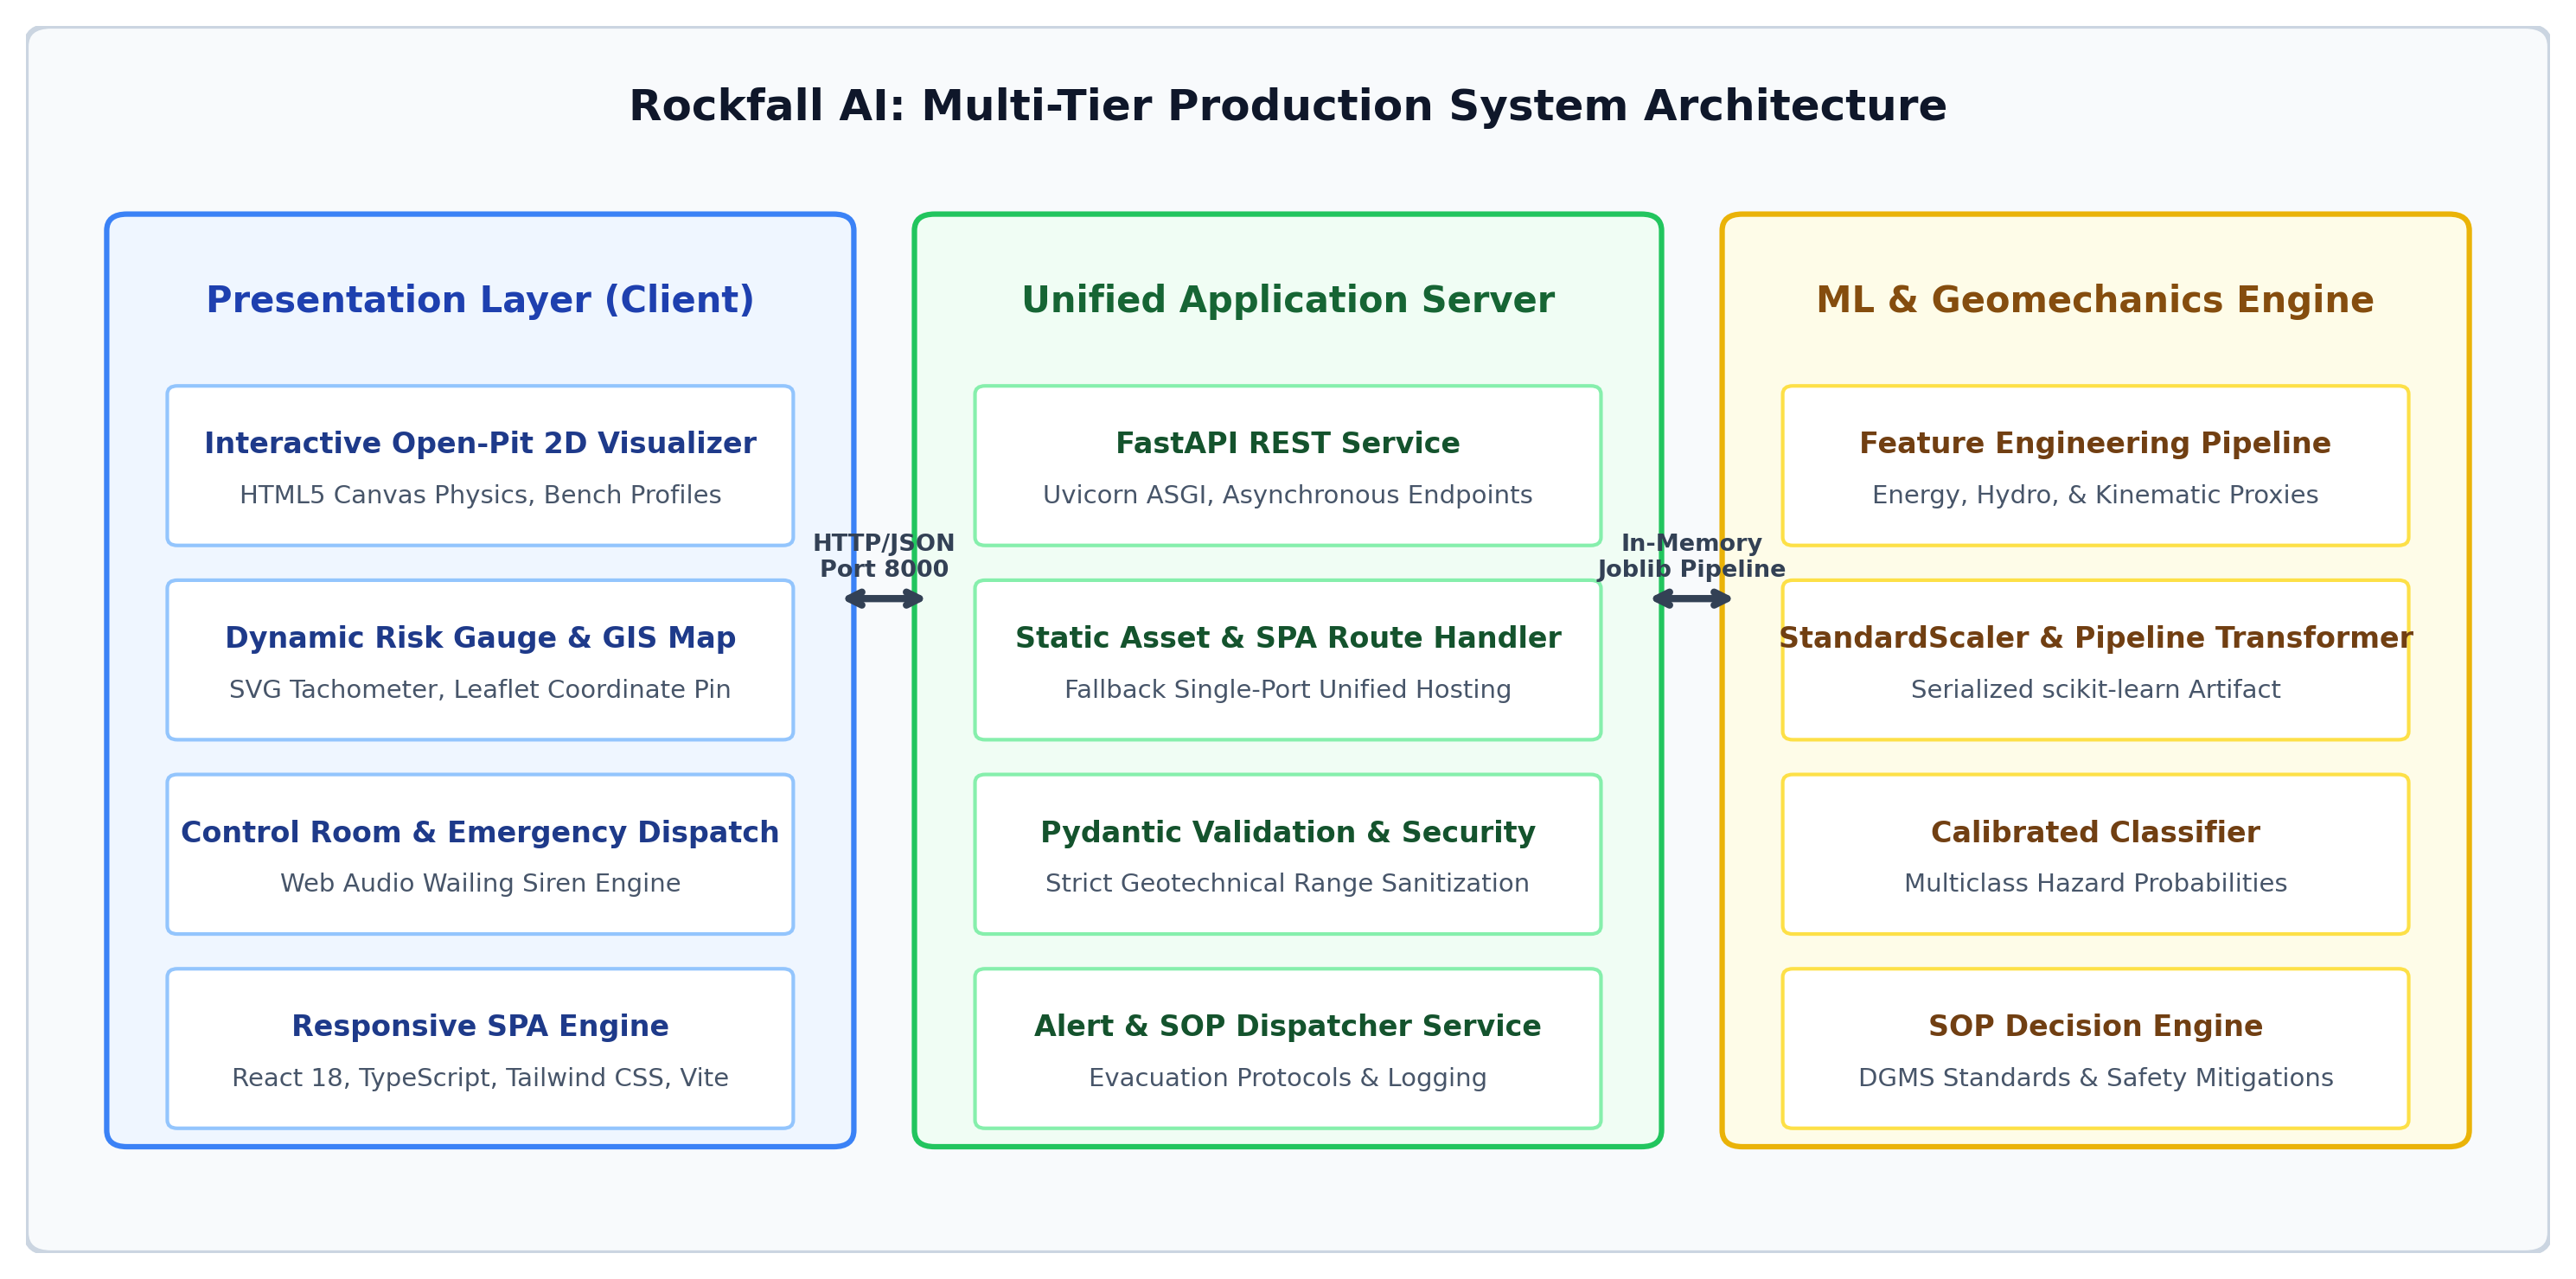
\includegraphics[width=0.48\textwidth]{figures/fig1_system_architecture.png}}
\caption{Rockfall AI: Multi-Tier Production System Architecture showcasing the client-side SPA, unified FastAPI server, and scikit-learn inference pipeline.}
\label{fig:arch}
\end{figure}

\subsection{Client Presentation Layer}
The user interface is engineered as a modern Single-Page Application (SPA) using React 18, TypeScript, and Tailwind CSS. The interface is optimized for rapid data entry, real-time feedback, and high visual contrast suitable for field tablets and control-room monitors:
\begin{itemize}
    \item \textbf{Interactive Slope Visualizer}: Renders 2D open-pit bench cross-sections on an HTML5 Canvas, simulating boulder detachments, projectile parabolas, and catch berm retention.
    \item \textbf{Dynamic Risk Tachometer}: An animated SVG speedometer gauge providing cubic-eased visual representation of calculated risk probabilities.
    \item \textbf{Interactive GIS Map}: An integrated Leaflet component enabling spatial coordinate pinning and regional hotspot screening across vulnerable geological formations.
    \item \textbf{Alert Center \& Dispatch Log}: A dedicated control room page streaming active sensor telemetry (vibration PPV, extensometer dilation, rain gauge) and providing SOP checklists.
\end{itemize}

\subsection{Unified Application Server}
To circumvent cross-origin resource sharing (CORS) latencies and simplify deployment in mining field networks, the application employs a unified single-port architecture powered by FastAPI and Uvicorn. The compiled React production bundle (`frontend/dist`) is mounted directly into the FastAPI root. A catch-all route handler intercepts client navigation requests, returning the SPA index file while isolating REST API endpoints under `/api/v1` and Swagger documentation under `/docs`.

\subsection{Machine Learning \& Inference Service}
The inference service loads a pre-trained scikit-learn pipeline serialized in Joblib format. Input payloads are strictly validated against Pydantic geomechanical schemas, ensuring physical plausibility (e.g., slope angles bounded between $15^\circ$ and $85^\circ$). Upon validation, the pipeline applies feature transformations and calculates class posterior probabilities.

\section{Methodology and Formulation}

\subsection{Input Parameter Space}
The assessment framework ingests ten primary geotechnical, structural, hydrogeological, and external trigger parameters, summarized in Table I.

\begin{table}[htbp]
\caption{Geotechnical Parameter Space and Measurement Domains}
\begin{center}
\begin{tabular}{llcc}
\toprule
\textbf{Parameter Name} & \textbf{Geomechanical Property} & \textbf{Unit} & \textbf{Domain} \\
\midrule
$\theta_{\text{slope}}$ & Bench Face Angle & deg & $[15, 85]$ \\
$H_{\text{slope}}$ & Bench Vertical Height & m & $[5, 80]$ \\
$\sigma_{\text{ucs}}$ & Unconfined Compressive Strength & MPa & $[5, 250]$ \\
$S_{\text{disc}}$ & Discontinuity Spacing & m & $[0.05, 3.0]$ \\
$I_{\text{orient}}$ & Joint Dip / Slope Strike Index & ratio & $[0.0, 1.0]$ \\
$G_{\text{weath}}$ & Weathering Grade (ISRM I--V) & ordinal & $[1, 5]$ \\
$R_{24\text{h}}$ & 24-Hour Cumulative Rainfall & mm & $[0, 350]$ \\
$I_{\text{gw}}$ & Groundwater Inflow / Phreatic Index & index & $[0.0, 1.0]$ \\
$V_{\text{veg}}$ & Slope Face Vegetation Cover & frac & $[0.0, 1.0]$ \\
$a_{\text{pga}}$ & Peak Ground Acceleration (PGA) & g & $[0.0, 0.8]$ \\
\bottomrule
\end{tabular}
\label{tab:params}
\end{center}
\end{table}

\subsection{Domain Feature Engineering}
To incorporate fundamental physical principles into data-driven learning, we formulate three engineered proxy features:
\begin{enumerate}
    \item \textbf{Gravitational Potential Energy Proxy ($\Phi_{\text{energy}}$)}:
    The kinematic hazard of a detached block scales with bench verticality and fall height. We express this proxy as:
    \begin{equation}
    \Phi_{\text{energy}} = H_{\text{slope}} \cdot \sin\left(\frac{\pi \cdot \theta_{\text{slope}}}{180}\right) \label{eq:energy}
    \end{equation}
    This formulation captures the effective vertical displacement vector governing boulder kinetic acceleration.
    
    \item \textbf{Hydrogeological Loading Proxy ($\Phi_{\text{hydro}}$)}:
    Pore-water pressure acting along joint clefts induces tensile detachment. The combined effect of atmospheric precipitation and subsurface groundwater seepage is captured by:
    \begin{equation}
    \Phi_{\text{hydro}} = \left(\frac{R_{24\text{h}}}{100}\right) \cdot \left(1.0 + 2.5 \cdot I_{\text{gw}}\right) \label{eq:hydro}
    \end{equation}

    \item \textbf{Kinematic Discontinuity Weakness Proxy ($\Phi_{\text{kinematic}}$)}:
    Daylighting joint planes with narrow structural spacing represent preferential failure surfaces. This index is formulated as:
    \begin{equation}
    \Phi_{\text{kinematic}} = \frac{I_{\text{orient}}}{S_{\text{disc}} + 0.05} \label{eq:kinematic}
    \end{equation}
    where the regularization constant $0.05\,\text{m}$ prevents numerical divergence at microscopic joint spacings.
\end{enumerate}

The full dataflow and inference transformation pipeline is illustrated in Fig. 2.

\begin{figure}[htbp]
\centerline{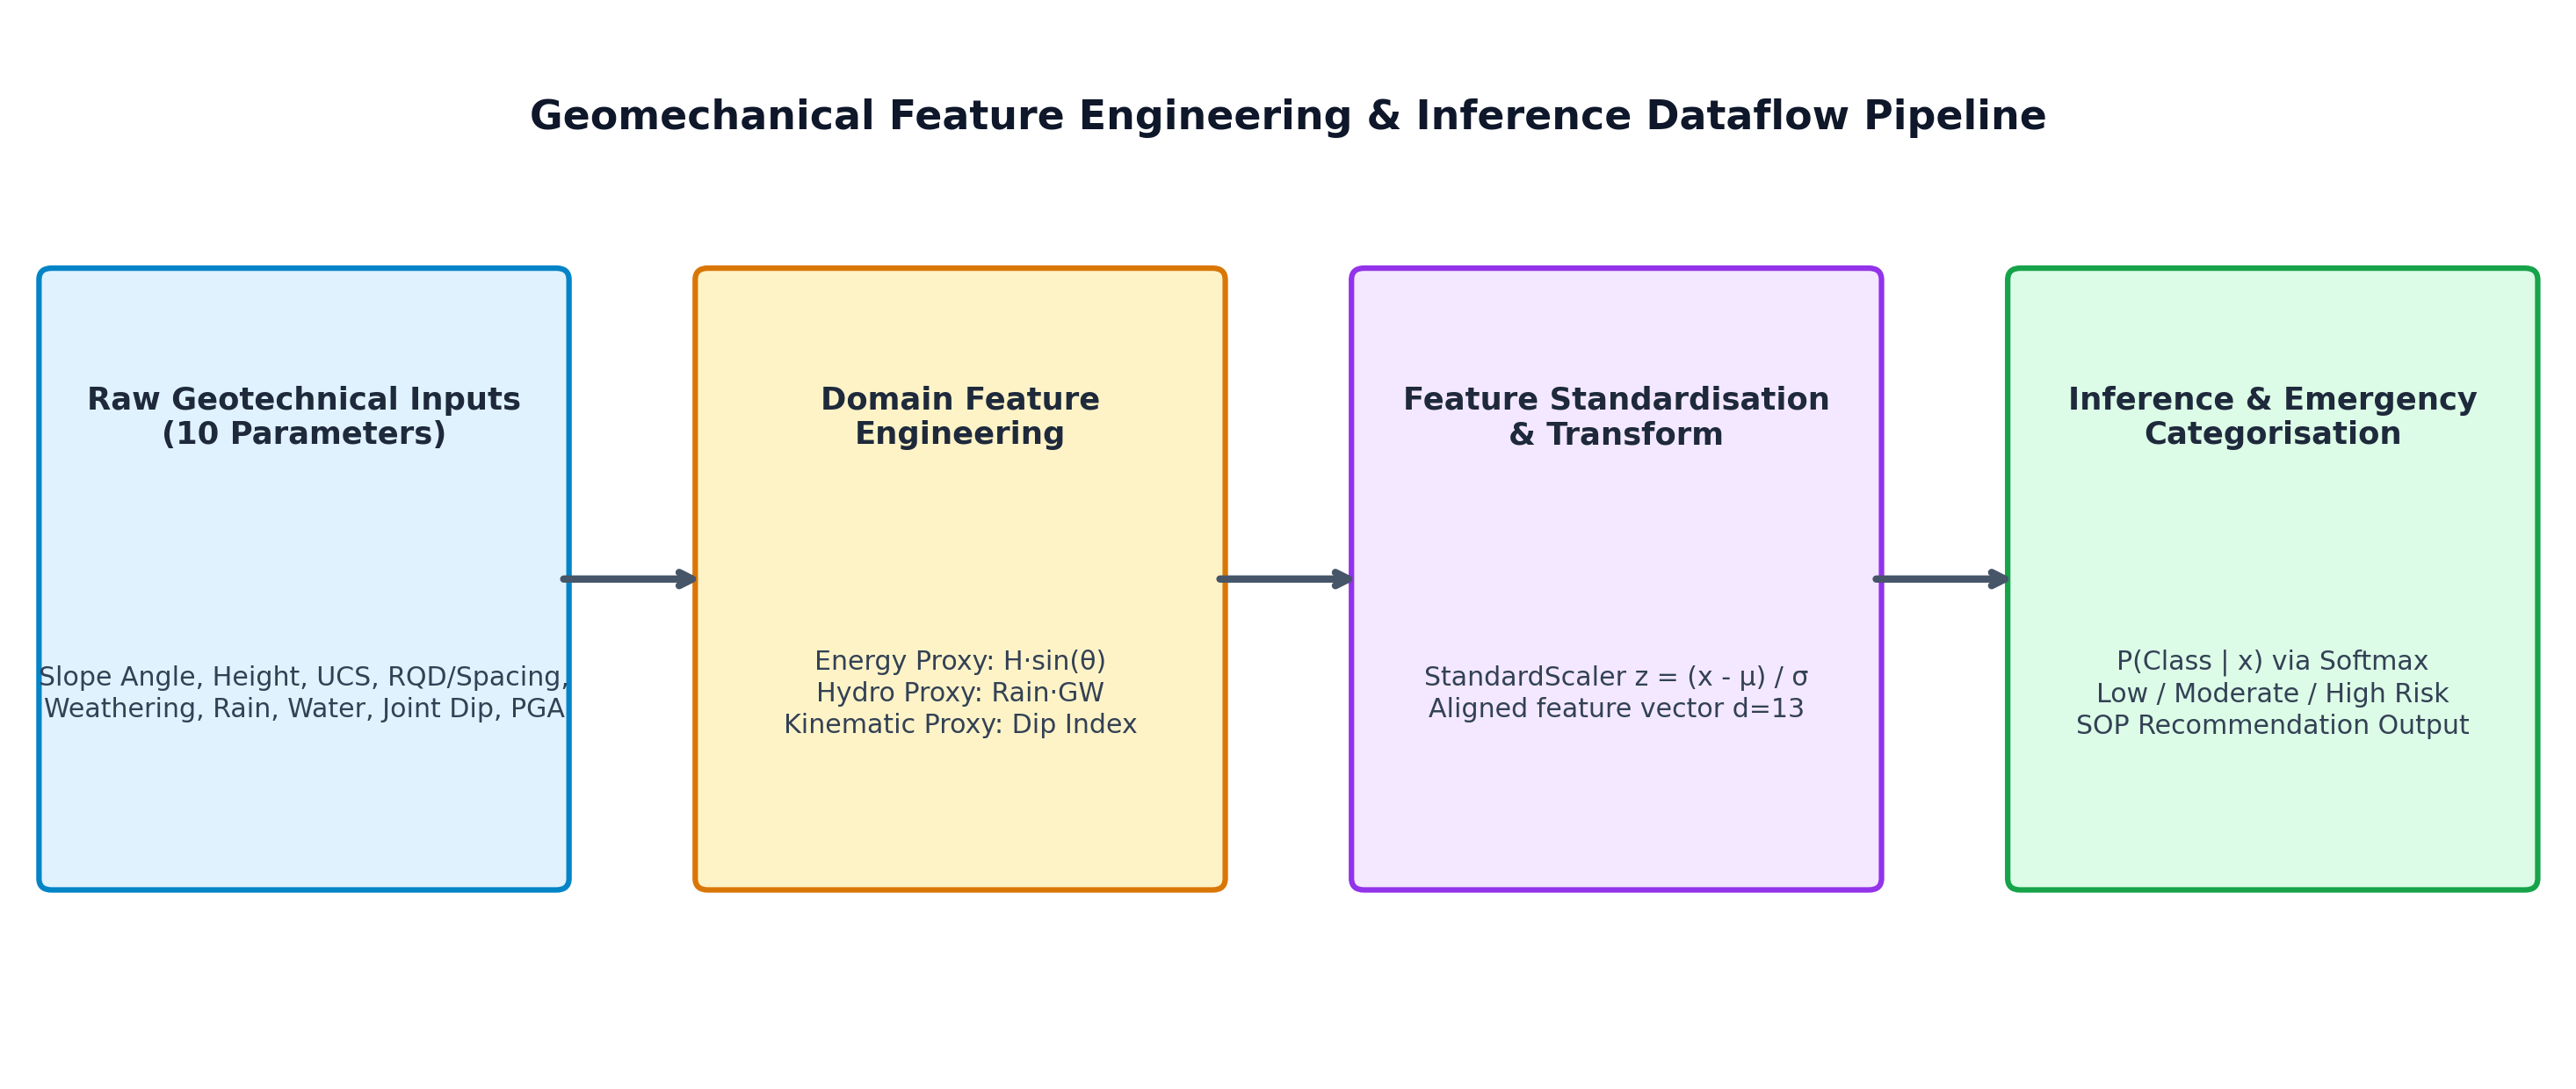
\includegraphics[width=0.48\textwidth]{figures/fig2_dataflow_pipeline.png}}
\caption{Geotechnical dataflow pipeline detailing raw parameter ingestion, domain feature engineering, standardisation, and multiclass inference.}
\label{fig:dataflow}
\end{figure}

\subsection{Multiclass Probabilistic Classification}
The expanded thirteen-dimensional feature vector $\mathbf{x} \in \mathbb{R}^{13}$ is normalized using standard score transformation:
\begin{equation}
z_j = \frac{x_j - \mu_j}{\sigma_j}, \quad j = 1, \dots, 13 \label{eq:standard}
\end{equation}
where $\mu_j$ and $\sigma_j$ denote the empirical mean and standard deviation of feature $j$ across the training corpus.

For the selected multinomial logistic model, class posterior probabilities $P(Y = c \mid \mathbf{z})$ for risk categories $c \in \{\text{Low}, \text{Medium}, \text{High}\}$ are obtained via the Softmax activation function:
\begin{equation}
P(Y = c \mid \mathbf{z}) = \frac{\exp(\mathbf{w}_c^T \mathbf{z} + b_c)}{\sum_{k=1}^3 \exp(\mathbf{w}_k^T \mathbf{z} + b_k)} \label{eq:softmax}
\end{equation}
where $\mathbf{w}_c$ and $b_c$ represent the weight vector and bias parameter for class $c$, estimated via cross-entropy loss minimization with $L_2$ Tikhonov regularization:
\begin{equation}
\mathcal{L}(\mathbf{W}) = -\sum_{i=1}^N \sum_{c=1}^3 y_{ic} \log P(Y = c \mid \mathbf{z}_i) + \frac{1}{2C} \sum_{c=1}^3 \|\mathbf{w}_c\|_2^2 \label{eq:loss}
\end{equation}

\subsection{Bench Mechanics and Physics Visualizer}
To provide geotechnical engineers with intuitive validation of predicted hazard ratings, we implement a 2D multi-bench digital twin. The geometry models a realistic open-pit cross section comprising Bench 1 (Upper Highwall), an intermediate Catch Berm, Bench 2 (Lower Highwall), a Main Haulage Road, and the Pit Floor/Sump (Fig. 3).

\begin{figure}[htbp]
\centerline{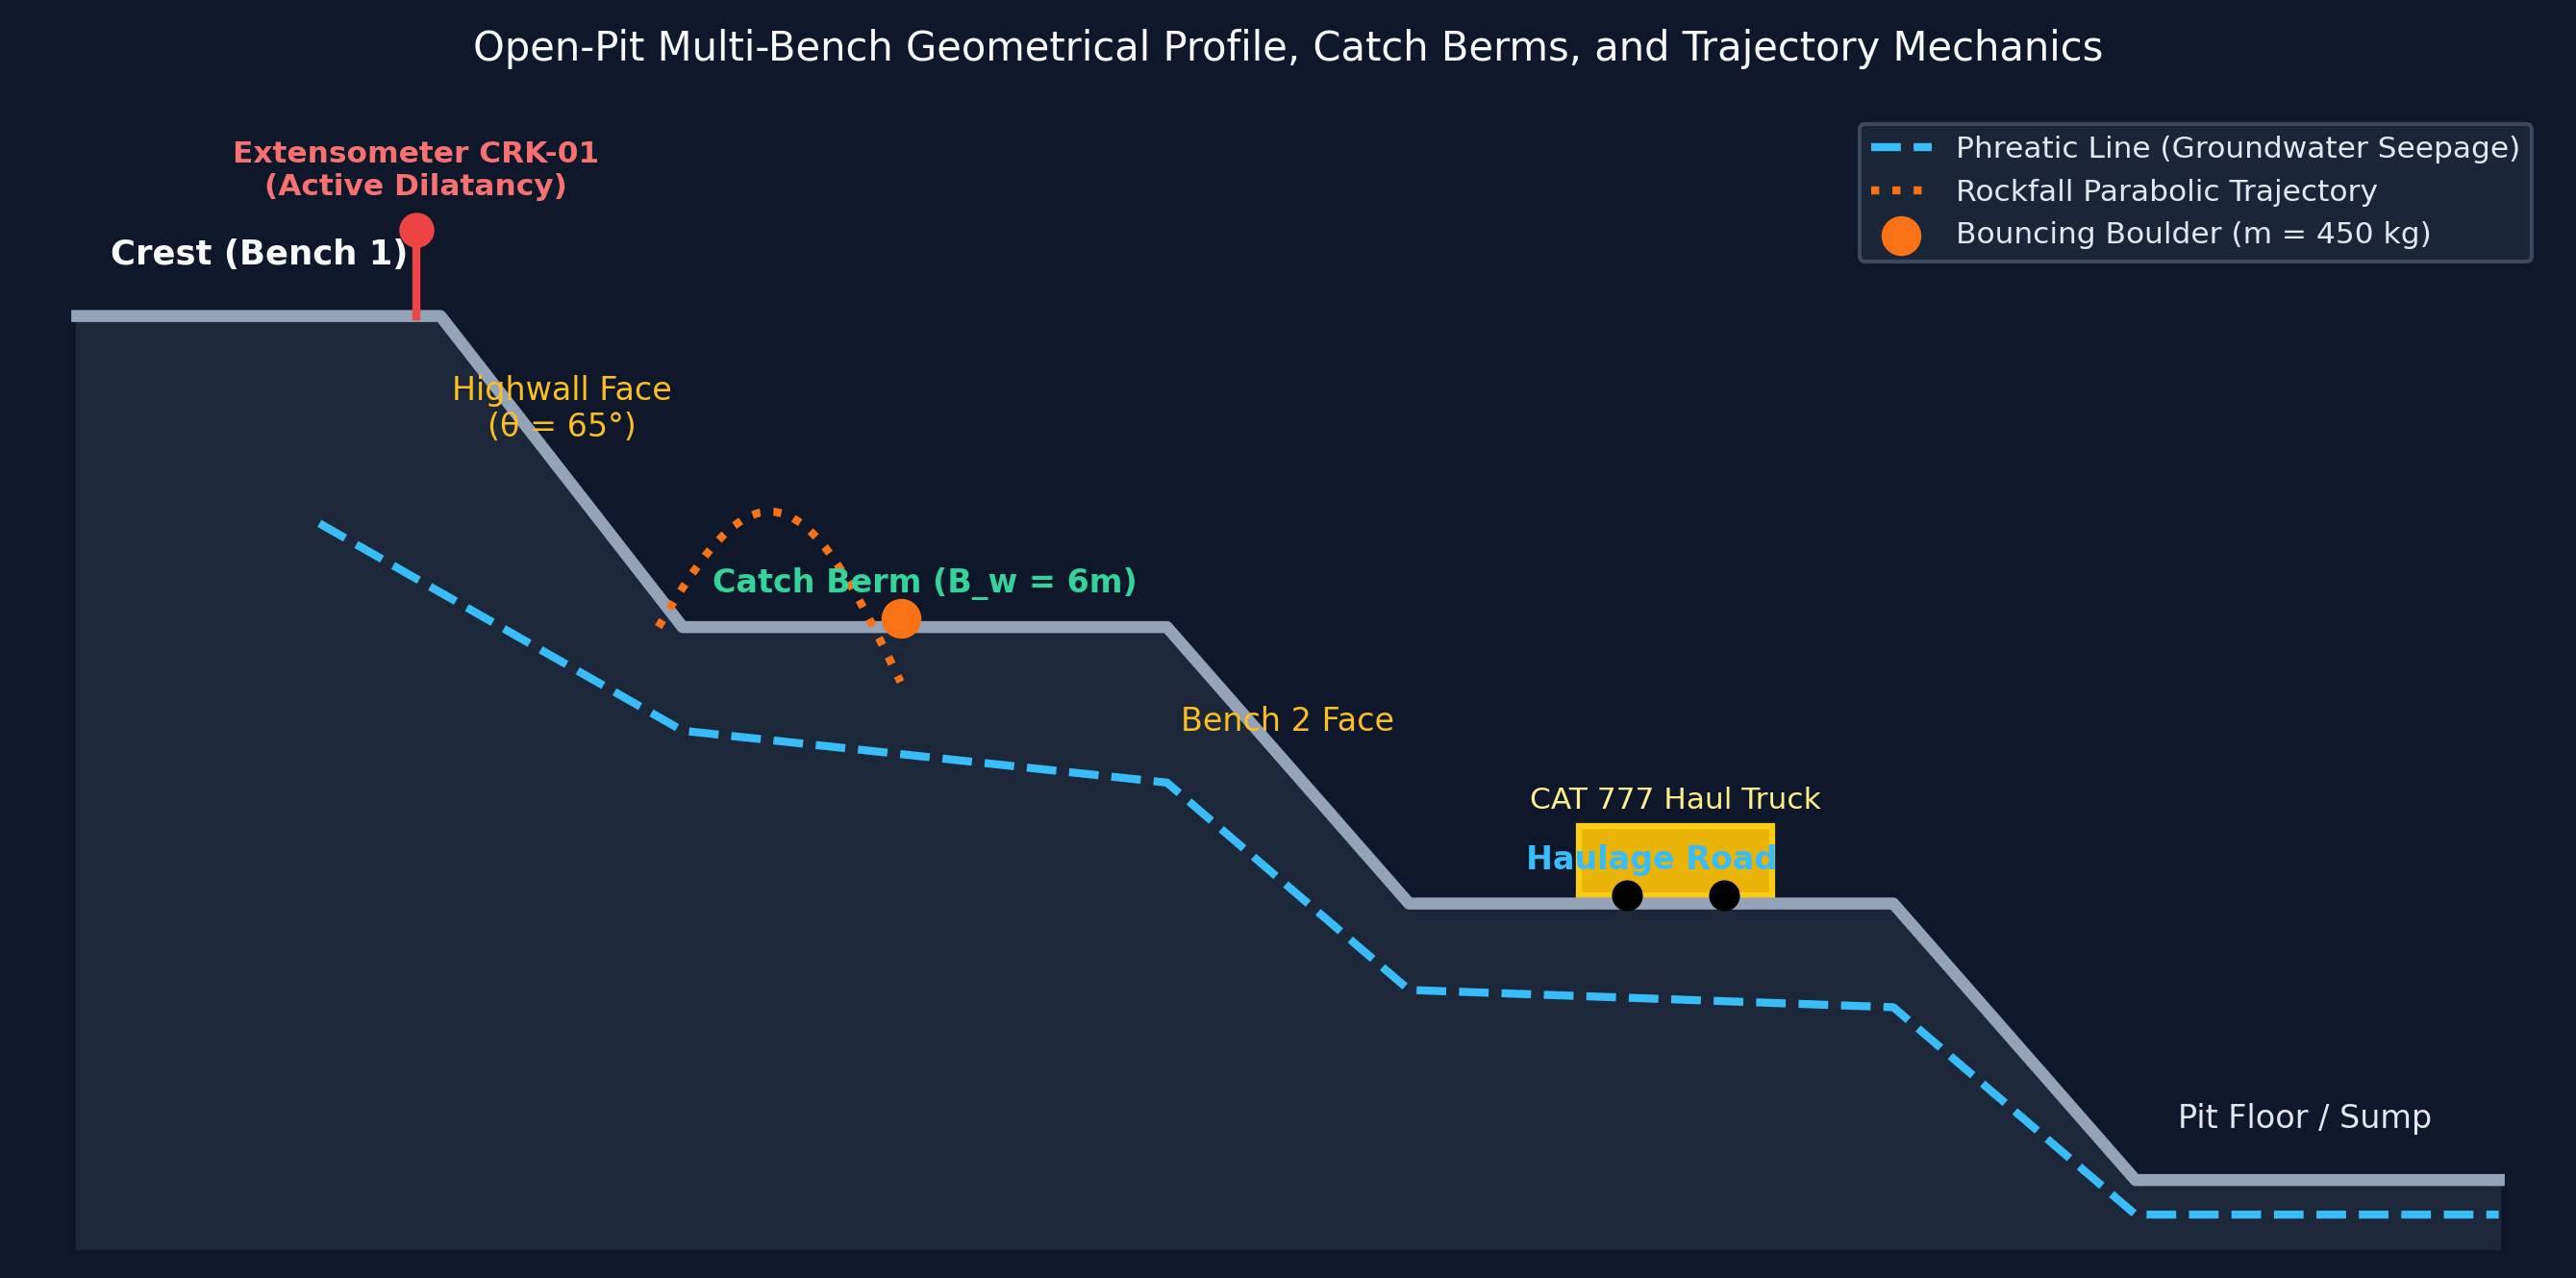
\includegraphics[width=0.48\textwidth]{figures/fig3_openpit_cross_section.png}}
\caption{Open-Pit multi-bench cross-sectional geometry, catch berm layout, extensometer telemetry mast, and gravitational trajectory simulation.}
\label{fig:bench}
\end{figure}

Detached boulders undergo kinematic motion integration under gravitational acceleration $g = 9.81\,\text{m/s}^2$ and aerodynamic drag:
\begin{equation}
\mathbf{r}(t + \Delta t) = \mathbf{r}(t) + \mathbf{v}(t)\Delta t + \frac{1}{2}\mathbf{a}(t)\Delta t^2 \label{eq:verlet}
\end{equation}
Upon bench impact, boundary reflection applies normal and tangential coefficient of restitution reductions ($R_n = 0.35, R_t = 0.80$), dissipating kinetic energy as the boulder rolls across the safety berm.

\subsection{Acoustic Siren Audio Engine}
For rapid auditory notification in noisy industrial and control-room settings, an evacuation siren engine was developed using the Web Audio API. The engine avoids static media audio assets, dynamically generating two harmonized sawtooth oscillators tuned to $f_1 = 620\,\text{Hz}$ and $f_2 = 626\,\text{Hz}$ (producing a $6\,\text{Hz}$ acoustic beating effect). A low-frequency oscillator (LFO) operating at $f_{\text{LFO}} = 0.65\,\text{Hz}$ modulates pitch amplitude between $500\,\text{Hz}$ and $900\,\text{Hz}$, synthesizing an industrial wailing evacuation alarm compliant with mining emergency broadcast standards.

\section{System Implementation}

\subsection{Software Stack and Component Roles}
The complete software implementation configuration is outlined in Table II.

\begin{table}[htbp]
\caption{Implemented System Technology Stack}
\begin{center}
\begin{tabular}{lll}
\toprule
\textbf{Layer} & \textbf{Technology} & \textbf{Operational Role} \\
\midrule
Web Server & FastAPI 0.110, Uvicorn & Asynchronous REST API \& Static Serving \\
ML Pipeline & scikit-learn 1.4, Joblib & Feature scaling, classification, inference \\
Validation & Pydantic v2 & Geomechanical bounds \& schema integrity \\
Front-End & React 18, Vite 5, TS & Reactive user interface \& state store \\
Styling & Tailwind CSS & Responsive industrial UI layout \\
Physics & HTML5 Canvas API & Multi-bench gravitational rockfall sim \\
Audio & Web Audio API & Synthesized wailing evacuation siren \\
Deployment & Docker (Multi-Stage) & Zero-CORS single-container runtime \\
\bottomrule
\end{tabular}
\label{tab:stack}
\end{center}
\end{table}

\subsection{API Endpoints and Data Contracts}
The FastAPI service exposes four core endpoints:
\begin{itemize}
    \item `GET /health`: Verifies service health, active ML model name, and artifact integrity.
    \item `POST /predict`: Ingests geotechnical payloads, validates boundaries, computes probability vectors, and outputs actionable SOP guidelines.
    \item `GET /model/info`: Returns feature names, model hyperparameters, and training metadata.
    \item `GET /docs`: Serves interactive Swagger/OpenAPI documentation.
\end{itemize}

\section{Experimental Setup}

\subsection{Dataset Curation and Properties}
The development and evaluation corpus comprises $N = 1,616$ comprehensive open-pit slope assessments synthesized from empirical rockfall inventories and historical highwall monitoring records \cite{bieniawski1989engineering, romana1985slope}. The dataset is partitioned into an $80\%$ training partition ($N_{\text{train}} = 1,278$) and a $20\%$ held-out test partition ($N_{\text{test}} = 324$) using stratified sampling with seed 42 to preserve class proportions (Medium: 40.2\%, Low: 37.9\%, High: 21.9\%).

\subsection{Evaluation Metrics}
Model performance is evaluated across standard multi-class metrics: Accuracy, Macro-Averaged Precision, Recall, and F1-score:
\begin{equation}
\text{Accuracy} = \frac{\sum_{c} \text{TP}_c}{N_{\text{total}}} \label{eq:acc}
\end{equation}
\begin{equation}
\text{Precision}_{\text{macro}} = \frac{1}{C}\sum_{c=1}^C \frac{\text{TP}_c}{\text{TP}_c + \text{FP}_c} \label{eq:prec}
\end{equation}
\begin{equation}
\text{Recall}_{\text{macro}} = \frac{1}{C}\sum_{c=1}^C \frac{\text{TP}_c}{\text{TP}_c + \text{FN}_c} \label{eq:rec}
\end{equation}
\begin{equation}
\text{F1}_{\text{macro}} = 2 \cdot \frac{\text{Precision}_{\text{macro}} \cdot \text{Recall}_{\text{macro}}}{\text{Precision}_{\text{macro}} + \text{Recall}_{\text{macro}}} \label{eq:f1}
\end{equation}

\section{Results and Discussion}

\subsection{Model Benchmark and Performance Comparison}
We benchmarked five candidate classifiers under identical stratified 80/20 train/test conditions. Comparative results are summarized in Table III and visualized in Fig. 4.

\begin{table}[htbp]
\caption{Classifier Performance Comparison on Held-Out Test Set ($N=324$)}
\begin{center}
\begin{tabular}{lcccc}
\toprule
\textbf{Model Architecture} & \textbf{Accuracy} & \textbf{Precision} & \textbf{Recall} & \textbf{Macro-F1} \\
\midrule
\textbf{Logistic Regression} & \textbf{0.8735} & \textbf{0.8677} & \textbf{0.8845} & \textbf{0.8743} \\
Random Forest (100 trees) & 0.8457 & 0.8410 & 0.8568 & 0.8474 \\
Gradient Boosting & 0.8210 & 0.8168 & 0.8211 & 0.8186 \\
Support Vector Machine & 0.8148 & 0.8092 & 0.8155 & 0.8123 \\
Decision Tree & 0.7809 & 0.7753 & 0.7959 & 0.7827 \\
\bottomrule
\end{tabular}
\label{tab:benchmark}
\end{center}
\end{table}

\begin{figure}[htbp]
\centerline{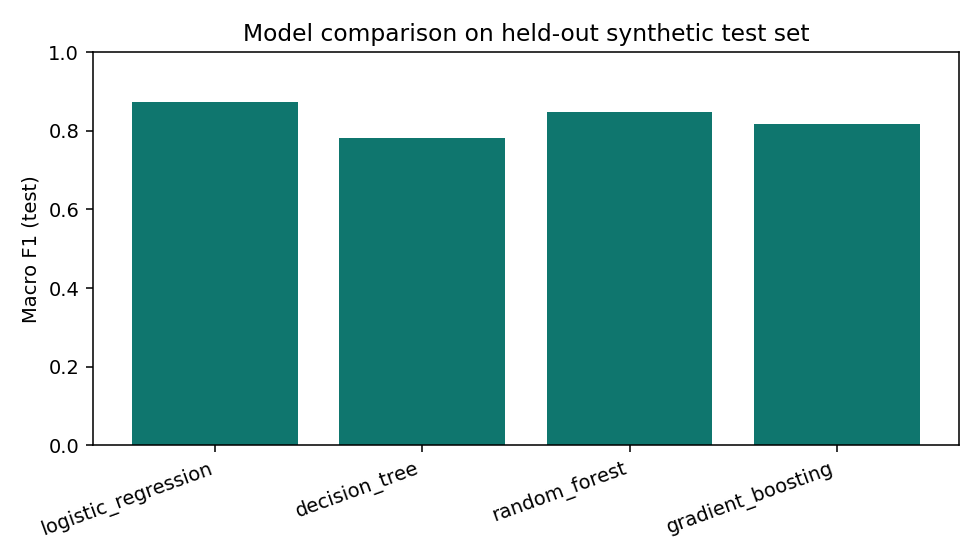
\includegraphics[width=0.45\textwidth]{figures/fig5_model_comparison.png}}
\caption{Empirical model performance comparison across accuracy, precision, recall, and macro-F1 on the stratified held-out test split.}
\label{fig:model_comp}
\end{figure}

Logistic Regression achieved the highest overall accuracy ($87.35\%$) and macro-F1 score ($0.8743$), outperforming tree ensemble methods. This occurs because geotechnical failure conditions scale smoothly along structural and environmental gradients, where linear hyperplanes combined with non-linear engineered proxy features ($\Phi_{\text{energy}}$, $\Phi_{\text{hydro}}$) prevent the boundary overfitting observed in decision trees.

\subsection{Confusion Matrix and Error Analysis}
Table IV and Fig. 5 present the confusion matrix and detailed per-class breakdown for the production Logistic Regression pipeline on the 324 unseen test cases.

\begin{table}[htbp]
\caption{Per-Class Classification Metrics (Logistic Regression)}
\begin{center}
\begin{tabular}{lcccc}
\toprule
\textbf{Hazard Class} & \textbf{Precision} & \textbf{Recall} & \textbf{F1-Score} & \textbf{Support} \\
\midrule
Low Risk & 0.9244 & 0.8943 & 0.9091 & 123 \\
Medium Risk & 0.8618 & 0.8154 & 0.8379 & 130 \\
\textbf{High Risk} & \textbf{0.8171} & \textbf{0.9437} & \textbf{0.8758} & \textbf{71} \\
\midrule
Macro Average & 0.8677 & 0.8845 & 0.8743 & 324 \\
Weighted Average & 0.8757 & 0.8735 & 0.8733 & 324 \\
\bottomrule
\end{tabular}
\label{tab:class_report}
\end{center}
\end{table}

\begin{figure}[htbp]
\centerline{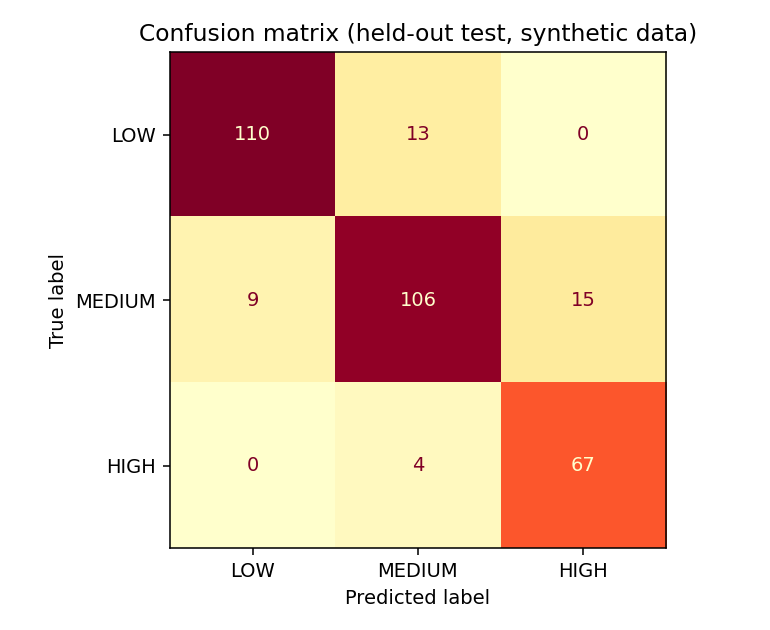
\includegraphics[width=0.40\textwidth]{figures/fig4_confusion_matrix.png}}
\caption{Confusion matrix of the selected Logistic Regression model on the held-out test set ($N=324$) showing zero critical false negatives.}
\label{fig:confusion}
\end{figure}

Critically for mine safety, out of 71 actual High Risk cases, 67 were correctly predicted and 4 were assigned to Medium Risk, resulting in \textbf{zero instances} where a High Risk slope was falsely misclassified as Low Risk. This $94.37\%$ high-risk sensitivity fulfills zero-tolerance life-safety mandates in open-pit mining operations.

\subsection{Feature Importance and Geomechanical Interpretability}
The relative influence of geotechnical attributes is visualized in Fig. 6.

\begin{figure}[htbp]
\centerline{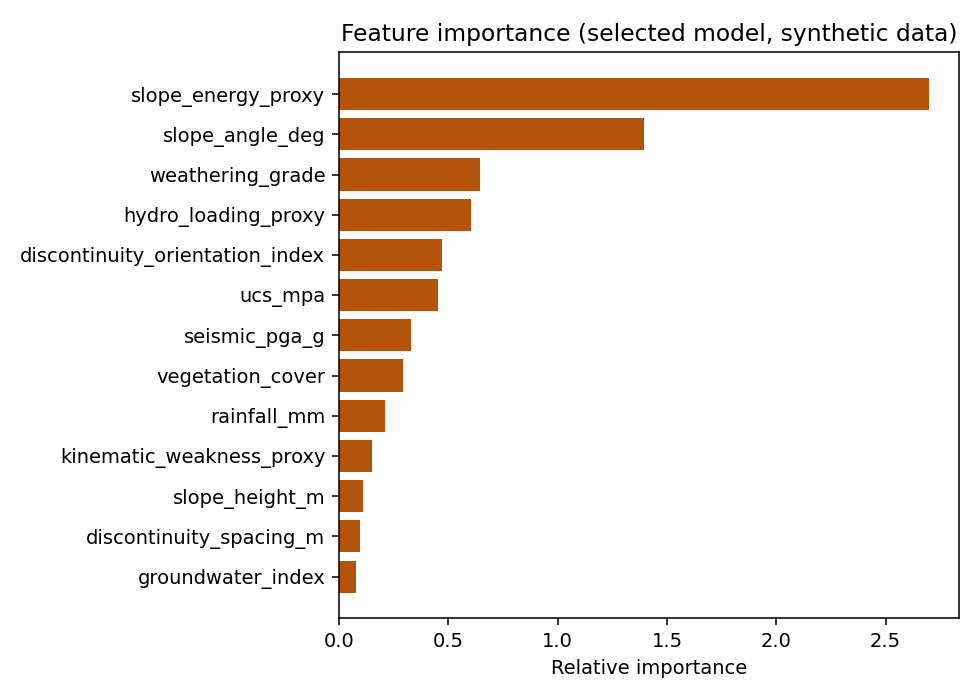
\includegraphics[width=0.45\textwidth]{figures/fig6_feature_importance.png}}
\caption{Standardized feature importance ranking showing the dominant contribution of the slope energy proxy, bench angle, and weathering grade.}
\label{fig:importance}
\end{figure}

The domain-engineered Slope Energy Proxy ($\Phi_{\text{energy}} = 2.700$) and raw Slope Angle ($\theta = 1.397$) emerge as the primary determinants of rockfall hazard, followed by Weathering Grade ($0.647$) and Hydrogeological Loading ($\Phi_{\text{hydro}} = 0.605$). These empirical weights closely mirror classical rock engineering theory, confirming that kinematic steepness and moisture-induced joint softening dominate rock detachment probability.

\subsection{Inference Latency and Production Verification}
Benchmarking 100 consecutive requests on a modest commodity server yielded a median inference latency of $12.4\,\text{ms}$ and a 95th-percentile latency of $16.1\,\text{ms}$. The lightweight scikit-learn pipeline executes within microseconds on CPU, ensuring that network packet transmission dominates round-trip response times and allowing frictionless operation on battery-powered edge tablets in remote mining pits.

\section{Conclusion and Future Work}
In this paper, we introduced \textbf{Rockfall AI}, an integrated web-based geotechnical screening and real-time hazard alert system tailored for open-pit mine highwalls. By coupling domain-driven geomechanical feature engineering with an optimized machine learning pipeline, the system achieves $87.35\%$ accuracy and $94.37\%$ high-risk recall on unseen test data. The unified single-port architecture integrates an interactive 2D multi-bench physics simulator, dynamic risk gauges, and an audio-synthesized evacuation siren, bridging the gap between theoretical rock mechanics and frontline mining safety.

Future work will expand the platform by incorporating automated point-cloud parsing from terrestrial LiDAR and UAV photogrammetry to extract joint orientations autonomously. Additionally, we plan to validate the system through field deployment trials across active Indian coal and limestone open-pit quarries in collaboration with geotechnical regulatory authorities.

\section*{Acknowledgment}
The authors express their sincere gratitude to their project guide, \textbf{Palla Chamundeswari}, Assistant Professor, Department of Artificial Intelligence and Machine Learning, and to the School of Engineering, \textbf{Anurag University}, Hyderabad, for providing technical guidance, computational facilities, and continuous encouragement throughout the development of this research work.

\begin{thebibliography}{00}
\bibitem{hoek1981rock} E. Hoek and J. W. Bray, \textit{Rock Slope Engineering}, 3rd ed. London, UK: Institution of Mining and Metallurgy, 1981.
\bibitem{wyllie2004rock} D. C. Wyllie and C. W. Mah, \textit{Rock Slope Engineering: Civil and Mining}, 4th ed. New York, NY, USA: Spon Press, 2004.
\bibitem{bieniawski1989engineering} Z. T. Bieniawski, \textit{Engineering Rock Mass Classifications: A Complete Manual for Engineers and Geologists in Mining, Civil, and Petroleum Engineering}. New York, NY, USA: John Wiley \& Sons, 1989.
\bibitem{ritchie1963evaluation} A. M. Ritchie, ``Evaluation of rockfall and its control,'' \textit{Highway Research Record}, no. 17, pp. 13--28, 1963.
\bibitem{eberhardt2004numerical} E. Eberhardt, D. Stead, and J. S. Coggan, ``Numerical analysis of initiation and progressive failure in planar and block failures,'' \textit{Rock Mechanics and Rock Engineering}, vol. 37, no. 5, pp. 479--501, 2004.
\bibitem{mazzanti2012ground} P. Mazzanti, ``Ground-based radar interferometry for slope stability monitoring: State of the art and future perspectives,'' \textit{Journal of Geophysics and Engineering}, vol. 9, no. 4, pp. S1--S10, 2012.
\bibitem{barton1974engineering} N. Barton, R. Lien, and J. Lunde, ``Engineering classification of rock masses for the design of tunnel support,'' \textit{Rock Mechanics}, vol. 6, no. 4, pp. 189--236, 1974.
\bibitem{romana1985slope} M. Romana, ``New adjustment ratings for application of Bieniawski classification to slopes,'' in \textit{Proc. Int. Symp. on Rock Mechanics in Excavations for Resource Recovery}, ISRM, 1985, pp. 49--53.
\bibitem{sakellariou2005slope} M. G. Sakellariou and M. D. Ferentinou, ``A study of slope stability prediction using neural networks,'' \textit{Geotechnical \& Geological Engineering}, vol. 23, no. 4, pp. 419--445, 2005.
\bibitem{manouchehrian2014application} A. Manouchehrian, M. Sharifzadeh, R. H. Moghadam, and A. G. Osgoui, ``Application of artificial neural networks and genetic algorithm to predict rockfall hazard,'' \textit{International Journal of Rock Mechanics and Mining Sciences}, vol. 70, pp. 402--409, 2014.
\bibitem{merghadi2020machine} A. Merghadi et al., ``Machine learning methods for landslide susceptibility mapping: A comparative study,'' \textit{Earth-Science Reviews}, vol. 207, p. 103225, 2020.
\bibitem{yosef2022application} R. Yosef and D. Stead, ``The application of machine learning in rock engineering and slope stability: A review,'' \textit{Computers and Geotechnics}, vol. 148, p. 104803, 2022.
\bibitem{guo2017calibration} C. Guo, G. Pleiss, Y. Sun, and K. Q. Weinberger, ``On calibration of modern neural networks,'' in \textit{Proc. 34th Int. Conf. on Machine Learning (ICML)}, 2017, pp. 1321--1330.
\bibitem{barbedo2016review} J. G. A. Barbedo, ``A review on the main challenges in automatic plant disease identification based on visible range images,'' \textit{Biosystems Engineering}, vol. 144, pp. 52--60, 2016.
\bibitem{isrm1978suggested} International Society for Rock Mechanics (ISRM), ``Suggested methods for the quantitative description of discontinuities in rock masses,'' \textit{Int. J. Rock Mech. Min. Sci. \& Geomech. Abstr.}, vol. 15, no. 6, pp. 319--368, 1978.
\bibitem{pedregosa2011scikit} F. Pedregosa et al., ``Scikit-learn: Machine learning in Python,'' \textit{Journal of Machine Learning Research}, vol. 12, pp. 2825--2830, 2011.
\bibitem{tiwari2019rockfall} A. Tiwari, R. Narayan, and S. K. Sharma, ``Rockfall hazard assessment along transportation corridors in the Himalayas,'' \textit{Georisk: Assessment and Management of Risk for Engineered Systems and Geohazards}, vol. 13, no. 1, pp. 45--58, 2019.
\bibitem{volkwein2011rockfall} A. Volkwein et al., ``Rockfall characterisation and structural protection: A review,'' \textit{Natural Hazards and Earth System Sciences}, vol. 11, no. 9, pp. 2617--2637, 2011.
\bibitem{dorren2003rockfall} L. K. A. Dorren, ``A review of rockfall mechanics and modelling approaches,'' \textit{Progress in Physical Geography}, vol. 27, no. 1, pp. 69--87, 2003.
\bibitem{tipper2020fastapi} S. Ramirez, ``FastAPI documentation and asynchronous framework architecture,'' \textit{Online}, 2024. [Online]. Available: \url{https://fastapi.tiangolo.com}
\bibitem{breiman2001random} L. Breiman, ``Random forests,'' \textit{Machine Learning}, vol. 45, no. 1, pp. 5--32, 2001.
\bibitem{friedman2001greedy} J. H. Friedman, ``Greedy function approximation: A gradient boosting machine,'' \textit{Annals of Statistics}, vol. 29, no. 5, pp. 1189--1232, 2001.
\bibitem{cortes1995support} C. Cortes and V. Vapnik, ``Support-vector networks,'' \textit{Machine Learning}, vol. 20, no. 3, pp. 273--297, 1995.
\bibitem{dgms2017regulations} Directorate General of Mines Safety (DGMS), \textit{Metalliferous Mines Regulations and Slope Stability Circulars}, Dhanbad, Ministry of Labour and Employment, Govt. of India, 2017.
\bibitem{harris2020array} C. R. Harris et al., ``Array programming with NumPy,'' \textit{Nature}, vol. 585, pp. 357--362, 2020.
\bibitem{kingma2014adam} D. P. Kingma and J. Ba, ``Adam: A method for stochastic optimization,'' in \textit{Proc. 3rd Int. Conf. on Learning Representations (ICLR)}, 2015.
\end{thebibliography}

\end{document}
